\documentclass[12pt]{article}
\usepackage[usenames,dvipsnames]{color}
\usepackage{listings}
\usepackage{graphicx}
\usepackage{fancyhdr}
\usepackage{framed}
\usepackage[T1]{fontenc}
\usepackage[toc,page]{appendix}
\usepackage[utf8]{inputenc}
\usepackage[brazil]{babel}
\usepackage{fancyvrb}
\usepackage[hmargin=2cm,vmargin=2cm]{geometry}
\usepackage{lastpage}
\usepackage{pdfpages}
\usepackage{makeidx}
\usepackage{hyperref}
\pagestyle{fancy}
\usepackage{enumitem}
% cabecalho e rodapé
\setlength{\headheight}{120pt}
\setlength{\textheight}{550pt}
\renewcommand{\headrulewidth}{0pt}
\lhead{
\includegraphics[scale=0.03]{brasao.png}}
%\chead{\includegraphics[scale=0.5]{logo-brasil-sem-pobreza2.png}}
\rhead{
\includegraphics[scale=0.5]{logo-pnud.png}}
\cfoot{\textbf{\ProjectCode\ - Inovando a democracia participativa}}
\rfoot{\thepage}

\hyphenation{par-ti-ci-pa-ção}
\bibliographystyle{ieeetr}

% definições sobre o autor e o produto
\newcommand{\MyName}{Renato Fabbri}
\newcommand{\MySurnameForename}{Fabbri, Renato}
\newcommand{\SupervisorName}{Ricardo Poppi}
\newcommand{\MyEmail}{renato.fabbri@gmail.com}
\newcommand{\ContractNumber}{2013/000566}
\newcommand{\ContractYear}{2014}
\newcommand{\ProjectCode}{Projeto BRA/12/018}
\newcommand{\NomeSecretaria}{Secretaria-Geral da Presidência da República}
%Q\newcommand{\SiglaSecretaria}{SG/PR}
\newcommand{\SiglaSecretaria}{Secretaria: SNAS }
\newcommand{\ProductNumber}{05}
\newcommand{\ProductTitle}{Proposta de regras de extração de conteúdos da API do portal e suas ferramentas para alimentação de eventual/hipotética base/nuvem de conhecimento de participação social}
\newcommand{\ProductSubtitle}{potencializando leituras focadas em incidência e participação social nas políticas públicas, com propostas de códigos}
\newcommand{\ProductDescription}{"Documento com proposta de regras de extração de conteúdos da API do portal e suas ferramentas para alimentação de eventual/hipotética base/nuvem de conhecimento de participação social potencializando leituras focadas em incidência e participação social nas políticas públicas, com propostas de códigos"}

\newcommand{\ProductValue}{R\$ 21,600 (vinte e um mil e seiscentos reais)}
\newcommand{\ObjetoContratacao}{
Aporte de conhecimentos e tecnologias para especificação de vocabulário e ferramentas assistidas que utilizam processamento de linguagem natural e análise de redes complexas para o conteúdo do portal da participação social.
}
\newcommand{\DataEntrega}{25 de Novembro de 2014}
\newcommand{\PalavrasChave}{reconhecimento de padrões, redes complexas, processamento de linguagem natural, web semântica, participação social}

% lista de abreviações
\makeindex
\begin{document}

\newgeometry{hmargin=3cm,vmargin=1.5cm}
\begin{center}
\thispagestyle{empty}
{\color{MidnightBlue}


\includegraphics[scale=0.9]{logo-pnud.png}

\vspace{4cm}

{\bf \large \ProjectCode\ - Desenvolvimento de Metodologias
de Articulação e Gestão de Políticas Públicas para Promoção da Democracia
Participativa}

\vspace{1.5cm}

{\bf \large Produto \ProductNumber\ -\ \ProductTitle}

\vspace{1.5cm}

\ProductSubtitle

\vspace{4cm}

\MyName

\vspace{1cm}

}


\includegraphics[scale=0.04]{brasao.png} \\
{\bf \small \NomeSecretaria}

\end{center}
\restoregeometry
\newpage

\newgeometry{hmargin=3cm,vmargin=1.5cm}
\addtolength{\topmargin}{2.5cm}
\thispagestyle{empty}
{\color{MidnightBlue}

{\bf \LARGE Produto \ProductNumber\ -\ \ProductTitle}

\hrulefill

\vspace{1cm}

\begin{center}

{\bf \large Contrato n. \ContractNumber}

\vspace{1.5cm}

{\bf \large Objeto da contratação: \ObjetoContratacao}

\end{center}

\vspace{3.2cm}

Valor do produto: \ProductValue

\vspace{1.2cm}

Data de entrega: \DataEntrega

\vspace{1.2cm}

Nome d@ consultor(a): \MyName

\vspace{1.2cm}

Nome d@ supervisor(a): \SupervisorName

}

\vspace{2cm}

\begin{center}

\includegraphics[scale=0.04]{brasao.png} \\
{\bf \small \NomeSecretaria}
\end{center}

\restoregeometry
\newpage

\newgeometry{hmargin=3cm,vmargin=1.5cm}
\addtolength{\topmargin}{5cm}
\thispagestyle{empty}

\begin{framed}

{\raggedright \MySurnameForename} \\

\ProductTitle: \ProductSubtitle\ / \ContractYear. \\

Total de folhas: \pageref{LastPage} \\

\vspace{1cm}

Supervisor(a): \SupervisorName \\

\SiglaSecretaria \\

\NomeSecretaria \\

Palavras-chave: \PalavrasChave. \\

\end{framed}

\vspace{3cm}

{\raggedright 
\includegraphics{licenca-cc-by-nc.png} \ Esta obra é licenciada sob
uma licença Creative Commons - Atribuição-NãoComercial. 4.0 Internacional.}

\restoregeometry
\newpage

\tableofcontents
\newpage


\begin{abstract}
Este documento descreve a alimentação com dados do Participa.br da nuvem de conhecimento de participação social. Não havia dados participativos brasileiros linkados, então a nuvem foi iniciada com a especificação ontológica e triplificação dos dados de duas outras instâncias: do AA, um sistema de compartilhamento de processos usado por programadores e midialivristas; e do Cidade Democrática, um portal participativo capitaneado pela sociedade civil. A triplificação do Participa.br e sua ontológia (OPa) foram feitas no primeiro e segundo produtos desta consultoria. Este trabalho aponta melhoras nesta integração do Participa.br aos dados linkados, com revisão de algumas estruturas iniciadas nesta consultoria e com o fornecimento de contexto.
{\bf Palavras-chave:} \PalavrasChave.
\end{abstract}
\newpage

\section{Introdução}

O termo de referência desta consultoria explicita para o quinto produto: \emph{regras de extração de conteúdos da API do portal e suas ferramentas para alimentação de eventual/hipotética base/nuvem de conhecimento de participação social}. A API do portal é o endpoint SparQL (RESTful). As ``regras de extração de conteúdos'' são ditadas pela linguagem SparQL em si, dadas as ontologias e os dados triplificados. A ontologia do participa (OPa) foi desenvolvida no primeiro produto desta consultoria, a triplificação entregue como parte do segundo produto~\cite{repoProd1, repoProd2}. Desta forma, este produto pôde se concentrar em melhorar esta alimentação da nuvem de conhecimento de participação social. Em especial, esta nuvem de participação social linkada via critérios semânticos e RDF é ainda incipiente e praticamente inexistente no contexto brasileiro. Isso motivou o desenvolvimento de duas novas ontologias de participação social: da \emph{Autorregulação Algorítmica}, uma técnica de compartilhamento de processos; e do \emph{Cidade Democrática}. Todas as tecnologias são livres e os links dos repositórios e softwares utilizados estão nos Apêndices.

\subsection{Contexto e importância da consultoria}
O portal federal de participação social (Participa.br) está imerso no contexto de redes, transparência e tecnologias em nuvem. Esta consultoria visa instrumentalizar a comunidade participativa brasileira, em especial em torno do Participa.br, para aproveitamento de nossas estruturas em rede, principalmente através de processamento de linguagem natural, redes complexas e dados linkados (vocabulários, ontologias e RDF). Este produto chega depois da disponibilização dos dados do Participa.br via critérios semânticos, nos produtos 1 e 2~\cite{repoProd1,repoProd2}. Também depois da exposição de formas de observação e de recomendação de recursos via técnicas de processamento de linguagem natural e redes complexas, nos produtos 3 e 4~\cite{repoProd3,repoProd4}. Neste produto foram reforçadas as frentes desta consultoria, embora os afazeres elencados como pertinentes e importantes sejam muitos (um detalhamento está em ~\url{https://etherpad.mozilla.org/prod5}). O objeto do produto já havia sido alcançado com os produtos anteriores e o consultor escolheu melhorar a triplificação atual do Participa.br e contemplar outras instâncias para potencializar (ou mesmo iniciar) a nuvem de participação social. Outro avanço foi o desenvolvimento das ontologias e vocabulários para a biblioteca (digital e semântica) de participação social, este bastante afinado com a equipe do Participa.br e outros andamentos da SNAS/SG-PR.

\subsection{Contexto e importância do produto}
Esta revisão da ontologia do Participa.br, triplificação dos dados do portal, levantamento de dados linkados da sociedade civil (AA e Cidade Democrática) e levantamento ontológico e de vocabulários linkados de interesse da SNAS/SG-PR (OBS e VBS), proporcionam qualidade e contexto para os dados linkados do Participa.br. Os dados são ditos ligados (linkados) pois estão em um formato com foco na interperabilidade, o ganho desta tecnologia é por vezes apontado como ``contexto para os dados''.

Há também um ganho de articulação para o Participa.br, que promoveu o desenvolvimento de tecnologias livres de ponta, com padrões internacionais incentivados via tratados, governos e sociedade civil de diversas origens. Mesmo assim, a importância para a articulação nacional é maior, contemplando interesses federais e civis.

\subsubsection{Objetivos}
O objetivo principal do trabalho foi integrar o Participa.br na nuvem de dados participativos linkados. Objetivos secundários foram:
\begin{itemize}
    \item Observar a incidência de outras ontologias de participação e de dados triplificados de outras instâncias participativas que não o Participa.br.
    \item Iniciar um repertório de dados participativos linkados brasileiros (\emph{bootstrap}).
    \item Articular partes interessadas neste legado aberto, tanto especializada (Participa.br), quanto envolvidas (SNAS/SG-PR com OBS e VBS e sociedade civil com AA e Cidade Democrática).
    \item Apresentar para as partes interessadas utilidades e possibilidades das tecnologias de web semântica.
\end{itemize}

\subsubsection{Resultados esperados}\label{subsec:resp}
Este trabalho auxiliou e deve continuar auxiliando a SNAS/SG-PR com respeito à biblioteca semântica e digital de participação social. A Ontologia da Biblioteca (semântica e digital de participação) Social, chamada OBS, e o Vocabulário da Biblioteca (semântica e digital de participação) Social, chamada VBS. Estas ontologias também devem facilitar a compreensão do funcionamento dos mecanismos e instâncias de participação social, tanto por iniciantes, como por gestores públicos ou acadêmicos especialistas, como apontaram alguns dos participantes do workshop realizado dia 20/10/2014.

Os dados do Participa.br já servem para mecanismos de recomendação de recursos, apresentados no produto 4 desta mesma consultoria~\cite{repoProd4}. Estes dados linkados estão já sendo disponibilizados por estruturas federais, mediante articulação da equipe do Participa.br. A ontologia do participa (OPa) contempla uma ontologia da concepção abstrata de portais participativos pela equipe do Participa.br. Com este produto, a OPa também contempla uma ontologia para o portal Participa.br, que possui classes e propriedades internas adequadas para representação dos dados do Participa.br. Estes desenvolvimentos podem ser aproveitados para proposições precisas de funcionamento do Participa.br, compartilhadas com relativa facilidade via diagramas e vocabulários em texto simples.

Os dados e ontologia do portal Cidade Democrática devem ser aproveitados pela comunidade relacionada ao portal. Na realização destas triplificações, foi iniciado um método de construção de ontologias orientado aos dados, útil para qualquer portal que queira triplificar seus dados em RDF e usufruir de uma ontologia.

Os dados e ontologia do AA estão em uso pelo labMacambira.sf.net. Continuará permitindo experimentações rápidas, dada a simplicidade da ontologia. Há implementações do AA planejadas para fazerem uso direto do endpoint SparQL para realizar updates com mensagens no momento de envio.

Estas instâncias em conjunto possibilitam análises comparativas, utilidades multiplataforma e observação de qualidades de desenvolvimentos diferentes.

\subsubsection{Caráter inovador}
Os dados linkados em RDF estão em uso bastante difundido por grandes corporações e alguns setores governamentais de alguns países. A disponibilização de dados cinco estrelas, com as tecnologias de ponta para ontologias e vocabulário (OWL e SKOS) é já de cosiderável inovação. A triplificação de dados de instâncias participativas adicionais, para iniciar uma nuvem de dados participativos, é de caráter inovador explícito.

O trabalho pode contribuir para suprir a lacuna de conhecimento que existe sobre as instâncias e mecanismos de participação social. Vários dos especialistas apontaram a falta de formalização destes processos, cabendo muitas vezes aos estudiosos, que garimpam os materiais produzidos entregar sistematizações.

A SGPR pode desenvolver a capacidade institucional de compartilhar seus processos, documentos, relatórios, em tecnologias que priorizam a interoperabilidade, facilitando suas atividades no poder federal, com drásticos aumentos na documentação enquanto a burocracia é minimizada.
Outra capacidade institucional que a SGPR pode desenvolver é de capitanear desenvolvimentos de tecnologias livres e abertura de dados.

\section{Desenvolvimento}\label{sec:dev}

\subsection{Comparação entre planejamento inicial e resultados alcançados}
Este produto foi idealizado com bastante coisa, para revisar, contextualizar e efetivar os desenvolvimentos apontados nos produtos anteriores. Um detalhamento está em \url{https://etherpad.mozilla.org/prod5}. A maior parte deste trabalho, a OBS e a VBS, não estava prevista. Mesmo assim, algumas das metas iniciais foram atingidas:
\begin{itemize}
    \item A ontologia do aa (Ontologiaa) foi feita em OWL, com relações de hiperclasses e hiperpropriedades. Os dados do AA foram triplificados, tanto os do MySQL quanto os do MongoDB. A comunidade já está se movendo em direção ao desenvolvimento de interfaces que atualizam as triplas no momento do envio das mensagens, via update do SparQL. A Ontologiaa foi usada para testes de inferências em tempo de real no endpoint Jena. Os resultados foram otimistas, provaram que é possível contar com as inferências em tempo de execução, mas não para um portal, pois as queries feitas chegaram a demorar alguns segundos para resposta.
    \item A ontologia do Cidade Democrática foi feita em OWL, e os dados do portal foram triplificados.
    \item A revisão da triplificação do Participa.br foi estudada e está sendo implementada no momento de entrega deste produto. Um novo módulo da OPa é fruto desta triplificação, relacionando diretamente a ontologia à versão atual dos dados do portal.
    \item Foi feito um estudo de navegação de dados, pelo qual foi efetivada a derreferenciação de todas as ontologias e triplificações com URIs que começam com \url{http://purl.org/socialparticipation/}:
\begin{itemize}
    \item \url{http://purl.org/socialparticipation/opa}
    \item \url{http://purl.org/socialparticipation/ops}
    \item \url{http://purl.org/socialparticipation/vbs}
    \item \url{http://purl.org/socialparticipation/obs}
    \item \url{http://purl.org/socialparticipation/aa}
    \item \url{http://purl.org/socialparticipation/ocd}
\end{itemize}
\end{itemize}

Algumas metas adicionais foram atingidas, não previstas inicialmente:
\begin{itemize}
    \item Um método foi desenvolvido para construção de ontologia orientada aos dados. O método foi utilizado para a construção da Ontologia do Cidade Democrática, com todos os axiomas de propriedade e restrições de classe apresentados pelos dados.
    \item Testes sobre as máquinas de inferência do Jena foram feitos, constatando tempos de execução de alguns segundos, que devem ser considerados. Além disso, as máquinas de inferência adicionaram segundos até mesmo às buscas que não precisaram de inferência. Outro fato constatado é a diferença, também de alguns segundos, entre o uso de máquinas de inferência de complexidade diferente (por exemplo: queries com inferências de super classes e super propriedades RDFS demoram metade das queries com inferências em OWL).
    \item Foram desenvolvidas a Ontologia e o Vocabulário da Biblioteca Social (OBS, VBS), com entrevistas, workshop para receber contribuições, estudos de documentos específicos e consideração especial do Decreto 8.243.
\end{itemize}

Este trabalho foi feito em imersão, resultando em diversos artefatos conceituais e tecnológicos. Os links apresentados neste trabalho certamente levam a derivados e produtos menores ou mais áridos tecnicamente.

\subsection{Etapas de desenvolvimento anteriores a este produto}
\subsubsection{Sistematização ontológica da participação online}
Através de estudos e reuniões presenciais e online, a Ontologia de Participação Social (OPS) foi revisada~\cite{OPS} e a Ontologia do Participa.br (OPA) foi feita~\cite{OPA}.
\subsubsection{Triplificação dos dados do Participa.br}
Feito um script para triplificar os dados do Participa.br, ou seja, para o enriquecimento semântico e escrita em RDF dos dados em Postgresql da instância Noosfero do Participa.br~\cite{triplifica}.
\subsubsection{Levantamento do endpoint SparQL}\label{sec:sfoo}
Para uso dos dados triplificados, pode-se recorrer a diversos métodos de leitura e disponibilização. Um método-chave é a disponibilização dos dados RDF (\emph{triple store}) em um \emph{endpoint sparql}. Para os fins de testes, pesquisa e usos leves, está disponibilizado um endpoint SparQL em servidores de pesquisa da USP~\cite{endpoint}.
\subsubsection{Análises iniciais, modelos}
Análises dos dados do Participa.br foram abertas no IPython Notebook, com ênfase no texto produzido e nas redes formadas~\cite{repoProd3}.
\subsubsection{Sistema de recomendação de participante e recursos}
O quarto produto desta consultoria explicitou como recomendar amigos, participantes, artigos, comentários, ou seja, recursos em geral, a partir de recursos de referência. Assim, pode-se recomendar para um usuário possíveis amigos, assim como possíveis opositores ou pessoas que tem traços de vocabulário. Outro exemplo é a recomendação de artigos, dado um comentário ou postagem como referência.

Em essência, o sistema de recomendação de recursos explicitado e sugerido pelo consultor é um enriquecimento na navegação dos dados que:
\begin{itemize}
    \item Utiliza técnicas de Processamento de Linguagem Natural e de Redes Complexas e técnicas híbridas.
    \item Explicita os critérios utilizados para a recomendação.
    \item Entrega os algorítmos utilizados em interfaces para testes, como o IPython.
    \item As recomendações são feitas via um recurso de referência, um tipo de recurso a ser recomendado, um método de recomendação. A maioria dos métodos aceita também uma polarização: similaridade ou dissimilaridade.
    \item As recomendações são acompanhadas de explicações de potenciais aproveitamentos.
\end{itemize}

\subsection{Etapas de desenvolvimento deste produto}
\subsubsection{Triplificação do AA e construção da Ontologiaa}
Com especial atenção a relações de superclasse e super propriedade, permitiu diversos testes dada a simplicidade do sistema.
\subsubsection{Triplificação dos dados do Cidade Democrática e construção da OCD}
Com o desenvolvimento de um método de construção de ontologias voltado aos dados.
\subsubsection{Desenvolvimento da OBS e VBS}
Através de entrevistas, workshop e materiais de referência, para uso na Biblioteca (semântica e digital de participação) social.
\subsubsection{Estudo de navegação de dados linkados}
Por onde foi iniciado o uso do Pubby e do Webprotege apontado nos Apêndices.
\subsubsection{Revisão da triplificação de dados do Participa.br e da OPa}
Com o paradigma de namespace interno, ampliação dos dados triplificados inicialmente e módulo adicional da OPa para os dados do Participa.br.

\subsection{Justificativa, descrição detalhada e formas de aplicação do método}
Os dados em RDF e as organizações ontológicas são tecnologias recomendadas, em expansão, com boa aceitação, interoperabilidade e organização de conceitualizações.

O método usado neste trabalho foi um para as ontologias e triplificação do Cidade Democrática, do AA e do Participa.br. Outro para as Ontologia e Vocabulário da Biblioteca (semântica e digital de participação) Social (OBS e VBS).

Para a OBS e VBS, foram feitas entrevistas, um workshop para receber contribuições, estudo detalhado de documentações e uma consideração especial do Decreto 8.243. Este foi o método ocorrente em articulação com a SNAS/SG-PR. Com o número de pessoas envolvidas, o método não foi idealizado de antemão, mas foi moldado segundo as necessidades e possibilidades encontradas no processo.

Nos outros casos, os dados são triplificados, as classes e propriedades utilizadas na triplificação são organizadas ontologicamente. Este foi o método mais apropriado para as instâncias virtuais, pois, como os experimentos iniciais com a OPa e a triplificação dos dados do Participa.br mostratam, os dados do portal apresentam várias relações que não são tratadas diretamente pela comunidade envolvida, resultando em uma aplicação incompleta da ontologia e uma perda grande dos dados do portal caso a triplificação seja mantida dentro do escopo da ontologia.

\subsection{Justificativa, descrição detalhada e acesso das fontes}
No caso em que as fontes foram os dados das instâncias, estas não estão acessíveis diretamente. Por exemplo: os dados sobre os quais os portais Participa.br e Cidade Democrática operam não estão disponíveis diretamente, apenas através dos dados triplificados ou através da equipe destes portais.

No caso da OBS e VBS, as fontes foram entrevistas, um workshopt e documentos de referência, explicitados no Apêndice.

\section{Resultados alcançados}
Foram construídas a OBS e VBS para a biblioteca de participação social. Formatos adicionais foram desenvolvidos para visualização dos vocabulários em texto simples a pedido da consultora Carmen Romcy. Scripts foram escritos para construção de aquivo XML lido pelo DSpace. Exportações do Tematres foram feitas locais para entregar para utilização pela SNAS. Foram feitas as ontologias do AA e do Cidade Democrática e os dados destas instâncias foram triplificados. Experimentos foram feitos com as máquinas de inferência do Jena através do Fuseki. Uma interface foi levantada para derreferenciar todas as classes, propriedades e instâncias que possuem o prefixo \url{http://purl.org/socialparticipation/}. As ontologias foram disponibilizadas no Webprotege da Stanford para receberem comentários e para desenvolvimento coletivo. A triplificação dos dados do Participa.br foi revisada, resultando em um módulo adicional para a OPa. 

Todas os desenvolvimentos estão em repositórios abertos e detalhados nos Apêndices.
\subsection{Usos dos resultados}\label{sec:uso}
Estes resultados estão em uso pelas comunidades envolvidas. Há previsões de que este arcabouço seja usado para análises periódicas e comparativas. Os resultados aqui apresentados devem impulsionar a apropriação das tecnologias semânticas, verbais e em rede no Brasil, tanto pela sociedade civil quanto pelo Estado. A SNAS está fazendo alguns usos da OBS e VBS para a biblioteca social e provavelmente será intensificado este processo.

\section{Conclusão}
As novas ontologias e roteiros de triplificação integram mais profundamente o Participa.br através de seus dados e organização ontológica, 
tanto na estrutura do Estado, com a OBS e VBS, quanto nas estruturas da sociedade civil, com a Ontologiaa, OCD, e as triplificações dos dados do AA e Cidade Democrática.

A qualidade dos desenvolvimentos foi verificada através da disponibilização no endpoint SparQL, scripts que fazem consulta aos endpoint, inteface para derreferenciamento (pubby), visualizações em diagramas e listagens e disponibilização no Webprotege.

Este é o último produto desta consultoria. Está prevista uma organização de todos estes materiais para facilitar utilização dos produtos desenvolvidos, assim como para realizar circulações e depurações acadêmicas, principalmente através de artigos. O trabalho desenvolvido com a SGPR e vínculo PNUD foi, para o consultor, permeada de experiências de excelência e aprendizado, o que manterá o consultor em prontidão para maiores simbióses que o poder federal julgar apropriadas.

\subsection{Comentários, sugestões, recomendações}
O consultor preferiu administrar ferramentas de web semântica ele mesmo, o que é proveitoso para melhorar a qualidade do trabalho. Mesmo assim, para os desenvolvimentos previstos por esta consultoria, ou similares que virem, pode ser proveitoso alocar um administrador de sistema para subir os programas necessários e até ajudar na pesquisa de softwares existentes. Outro suporte pertinente é de um programador para facilitar e potencializar os desenvolvimentos em código. Outros profissionais (linguístas, cientístas da computação, estatísticos, etc) são também pertinentes, mas podem ser aproximados em regime de consultas remuneradas a vulso e mediante a necessidade.

Um fenômeno social envolvido no vínculo do consultor, que talvez deva ser considerado, é o de diminuição da adesão de colaboradores quando a consultoria é efetivada. Há diversos fatores envolvidos, em geral os parceiros consideram a aproximação do Estado como uma potencial distorção das posturas e andamentos. Isso facilita uma aproximação do consultor com o Estado, mas pode ser considerada uma razão a mais para providenciar possibilidades de remunerar algumas interações.

\subsection{Impacto do produto para a elaboração, gestão e/ou avaliação de políticas públicas de participação social}
Este produto pode impactar as políticas públicas através da organização do conhecimento, que facilitará a obtenção de informações mais expressivas.  Outro impacto previsto é relacionado à transparência, pois os dados linkados, além de abertos, está em constante conexão com o legado humano de dados linkados. A avaliação de políticas públicas contará com relatórios comparativos e periódicos, potencialmente automatizados, que instrumentalizarão os gestores. A eficiência e pertinência dos desenvolvimentos aqui apresentados devem colaborar substancialmente para uma consideração técnica mais profunda por parte dos gestores públicos, mas também de toda a sociedade.

A consideração de instâncias civís (inicialmente através da OCD e Ontologiaa), do Participa.br (OPa) e dos mecanismos e instâncias de participação social (OBS e VBS) tem como um dos propósitos principais impactar diretamente o gestor público com a disponibilização de informações navegáveis, interoperáveis e enriquecidas semanticamente.

\subsection{Impacto no público-alvo das políticas públicas}
As organizações ontológicas e dados triplificados facilitam análises periódicas, comparativas, recomendações de recursos, navegação de recursos e apreensão das informações relacionadas. Assim, há um empoderamento previsto do gestor e do cidadão interessado. Ao mesmo tempo, a transparência é reforçada. A apropriação das tecnologias em rede, em especial as ligadas ao processamento de linguagem natural, redes complexas e dados linkados, é potencializada com a disponibilização das tecnologias livres desenvolvidas nesta consultoria. Os vínculos e apoios do PNUD e da SGPR são eficientes para sinalizar ao gestor público e ao cidadão que estas tecnologias são proveitosas e devem ser apropriadas pela sociedade.


\section{Agradecimentos}
O consultor Renato Fabbri agradece ao Joenio Costa pelo template em \LaTeX\ para os produtos. Agradece a todos os conhecedores entrevistados, pois em muito ajudaram na realização deste produto. Agradece aos supervisores do trabalho realizado em torno do Participa.br: Ricardo Poppi e Ronald Costa. Agradece ao labMacambira.sf.net e todas as comunidades de software e cultura livre que compõe esta contribuição.
\newpage
\bibliography{bibliografia}
\newpage
%\listoffigures
\section*{Abreviações e jargão}
\begin{itemize}[label={}]
    \item {\bf RC:              } Redes Complexas
    \item {\bf PLN:             } Processamento de Linguagem Natural
    \item {\bf OPS:             } Ontologia de participação Social
    \item {\bf OPA:             } Ontologia do Participa.br
    \item {\bf MMISSA:          } Monitoramento Massivo e Interativo da Sociedade pela Sociedade para Aproveitamento
    \item {\bf AARS:            } A Análise de Redes Sociais
    \item {\bf MyNSA:           } Monitoring yields Natural Streaming and Analysis
    \item {\bf PNPS:            } Plano Nacional de Participação Social
    \item {\bf RDF:             } Resource Description Framework
    \item {\bf HTTP:            } Hypertext Transfer Protocol
    \item {\bf SPARQL:          } Simple Protocol and RDF Query Language
    \item {\bf endpoint SPARQL: } ponto de acesso, geralmente HTTP, a dados em RDF via buscas em SPARQL.
    \item {\bf Participa.br:    } Portal federal de participação social.
    \item {\bf IPython Notebook:} instância online para rodar scritps Python
    \item {\bf Meteor:          } arcabouço para páginas reativas e com funcionamento distribuído.
    \item {\bf D3js:            } biblioteca de visualização de dados.
\end{itemize}

\newpage
\printindex
\newpage
%\input{listadeanexos.tex}
\appendix
\section{Ontologias de instâncias participativas online potencialmente relacionáveis ao Participa.br}
\subsection{Ontologia do AA (Ontologiaa)}\label{ap:aa}
Como uma forma de integrar o Participa.br em uma nuvem de conhecimento participativo, foi levantada a Ontologiaa, exposta na Figura~\ref{fig:diaa}. O AA é uma técnica de compartilhamento de processos usada principalmente no labMacambira.sf.net. A simplicidade das implementações atuais, e a pertinência do registro e compartilhamento de processos, fizeram com que esta fosse o primeiro desenvolvimento efetivo deste último produto.

\begin{figure}[h!]
  \centering
    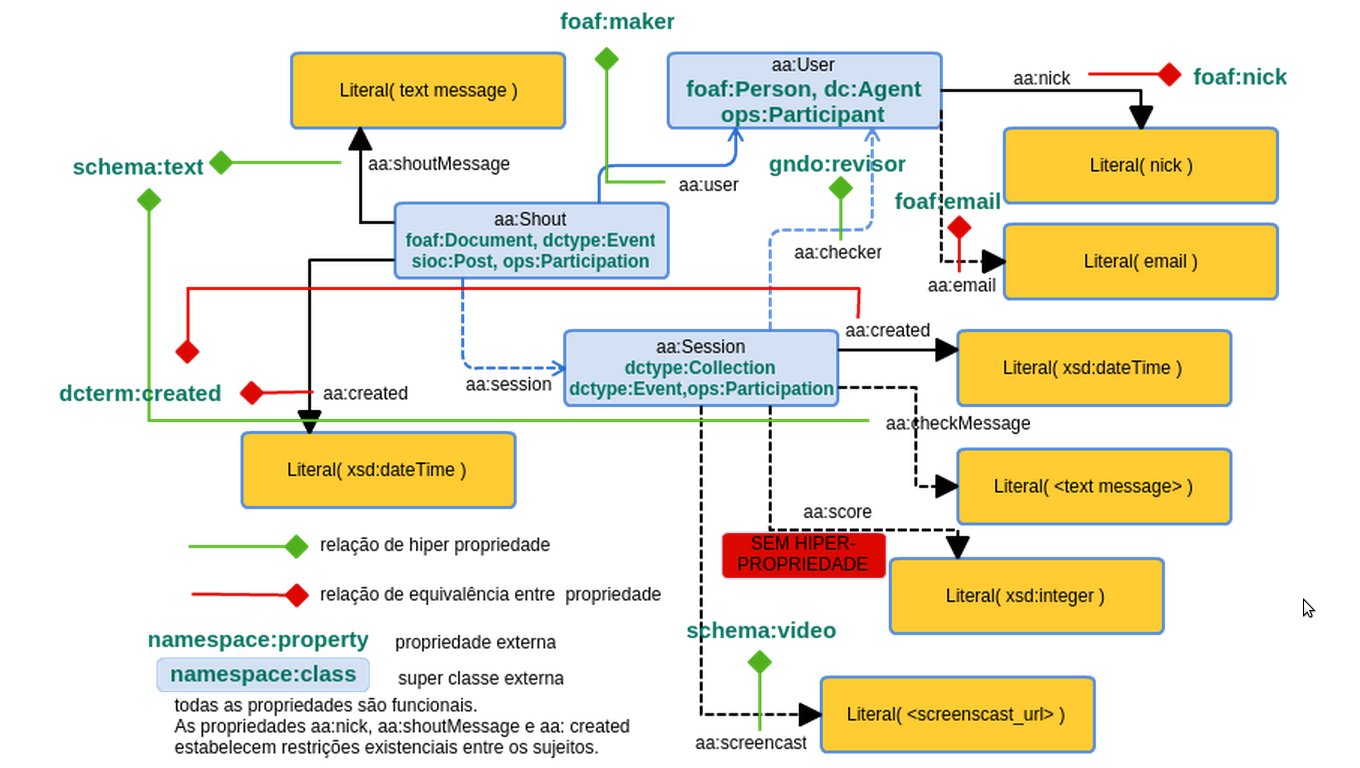
\includegraphics[width=\textwidth]{../figs/ontologiaa.png}
  \caption{Ontologia do AA, com suas classes, propriedades, literais, e classes e propriedades externas usadas para relacionar os dados do AA aos do participa e de toda nuvem LOD.}\label{fig:diaa}
\end{figure}

O tamanho reduzido da ontologia permitiu que vários testes fossem feitos. Em especial, com a ontologiaa foi reestabelecida a arquitetura de ontologia com uso de um namespace interno (no caso \url{http://purl.org/socialparticipation/aa/} e inferências para contemplar outros namespaces.

As inferências foram testadas com o jena/fuseki, com bons resultados. Tanto as inferências relacionadas às hiperonímias (superclasses e super propriedades, diretamente do rdfs) quanto inferências mais elaboradas (ligadas ao padrão OWL) foram satisfatórias. O revés é que qualquer query SparQL que demora milissegundos, mesmo que não envolva inferências para sua resposta, demora segundos quando há uma máquina de inferências ativa. A solução, portanto, parece ser ainda de realizar estas inferências offline e disponibilizar todas as triplas resultantes no endpoint.

Todos os desenvolvimentos desta ontologia e a triplificação de dados do AA em MySQL e MongoDB estão em: \url{https://github.com/ttm/aa01/tree/master/rdf}. Estes dados estão disponíveis no endpoint sparql (fuseki/jena) para uso conforme script ipython. Há interfaces úteis para explorar/expor os dados ligados ao AA. Em especial, estão derreferenciáveis, como na Figura~\ref{fig:aashout}.

\begin{figure}[h!]
  \centering
    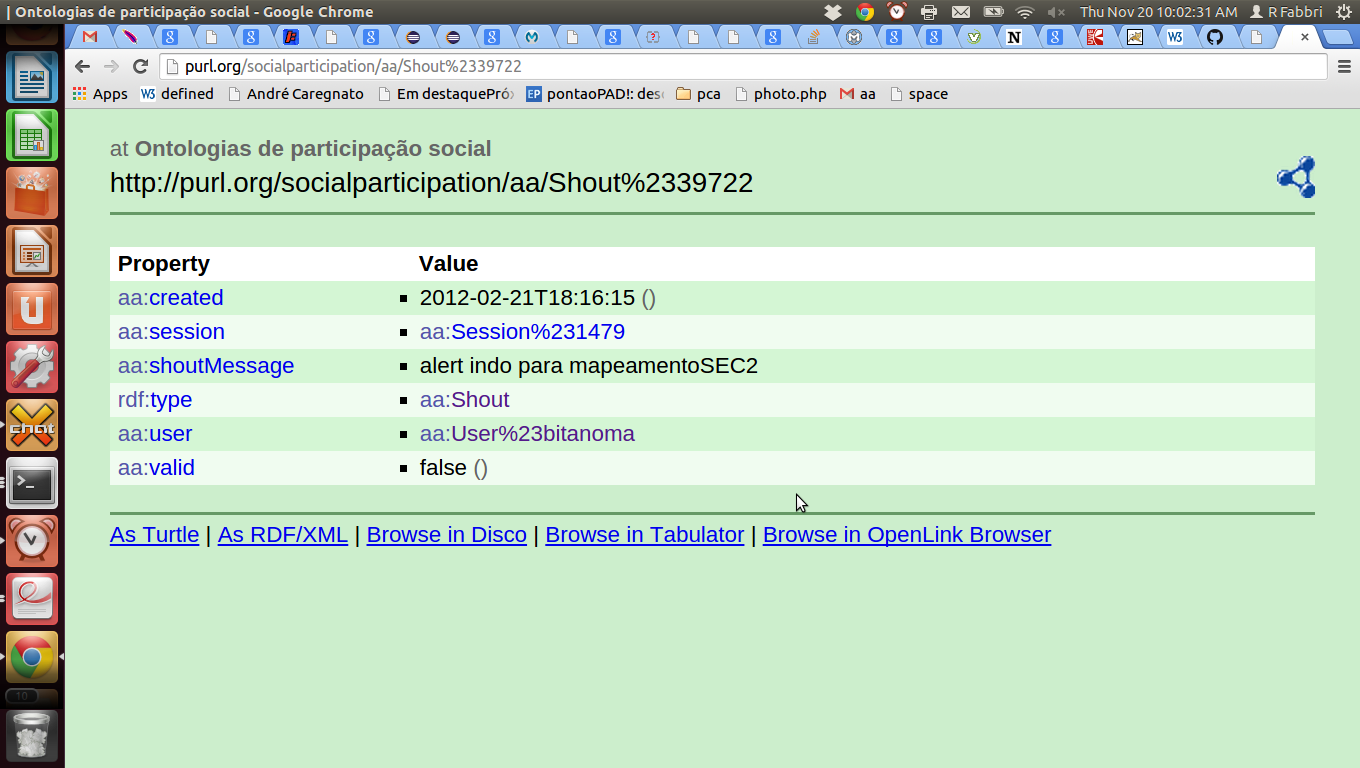
\includegraphics[width=\textwidth]{../figs/aaShoutPubby.png}
  \caption{Mensagem (shout) do AA derreferenciado. Cada mensagem do AA recebe uma URI, assim como cada sessão e cada usuário. Estes três conceitos são instânciados com URIs dedicadas, e relacionadas via ainda outras URIs. Por fim URIs especificam relações entre instâncias destes conceitos e os dados.}\label{fig:aashout}
\end{figure}

A ontologia do AA está no webprotege da Stanford~\url{http://webprotege.stanford.edu/#Edit:projectId=5207dd13-8706-4836-bad9-6cba1c81de29}.

\subsection{Ontologia do Cidade Democrática (OCD)}
Outra instância participativa considerada prioritária pelo consultor para integração aos dados participativos linkados, e contemplada neste trabalho, foi o portal Cidade Democrática. Este portal possui grande complexidade e abundância de dados e conceitos. Assim, esta empreitada contrastou com a da Ontologiaa descrita no Apêndice~\ref{ap:aa}.

Com a grande complexidade das tabelas e dados, foi feita uma decupagem do banco de dados (disponibilizada em \url{https://github.com/ttm/ocd/blob/master/decupagemBD.txt}) e uma triplificação destes dados (script em: \url{https://github.com/ttm/ocd/blob/master/triplificaCD.py} e triplas resultantes em \url{https://github.com/ttm/ocd/blob/master/cdTriplestore.rdf.tar.gz}).

Embora os trabalhos de decupagem do banco e de triplificação dos dados sejam expressivos, o ponto alto desta empreitada foi a gênese de um método de levantamento de ontologia orientado aos dados. Este método é extremamente útil para qualquer portal que queira representar seus dados como triplas RDF e uma ontologia. O processo é o seguinte:

\begin{enumerate}
    \item Todos os dados de interesse são triplificados com namespace interno, conforme: \url{https://github.com/ttm/ocd/blob/master/triplificaCD.py}.
    \item Os dados triplificados são disponibilizados em um endpoint sparql para levantamento da ontologia com base nas triplas produzidas (endpoint em: \url{http://200.144.255.210:8082/cd/query}).
    \item Um script é construído, no qual os dados triplificados são usados para observação das estruturas ocorrentes, conforme \url{https://github.com/ttm/ocd/blob/master/OCD.py}. Principalmente:
\begin{itemize}
        \item São observadas todas as classes ocorrentes.
        \item São observadas todas as propriedades ocorrentes.
        \item As propriedades são especificadas como funcionais e inversamente funcionais (axiomas de propriedade), conforme os dados apresentarem tais relações.
        \item As classes recebem restrições universais e existenciais, conforme os dados apresentarem estas relações.
        \item São feitas imagens de cada propriedade, com os elementos imediatamente relacionados a eles, como na Figura~\ref{fig:ocdp}.
        \item São feitas imagens de cada classe, com os elementos imediatamente relacionados a eles, como na Figura~\ref{fig:ocdc}.
        \item São feitas imagens diferentes da estrutura global, para facilitar apreensão da ontologia, como a Figura~\ref{fig:ocdg}.
        \item Ontologia OWL é escrita, conforme disponibilizada em: \url{https://github.com/ttm/ocd/blob/master/OCD.owl} ou \url{https://github.com/ttm/ocd/blob/master/OCD.ttl}.
        \item Os conceitos são relacionados a conceitos mais gerais, de ontologias externas, para facilitar a integração dos dados do portal com o grafo gigante e global~\cite{LOD}. Este passo não foi dado na OCD por limitação de tempo mesmo. Há outras prioridades e a comunidade deste portal está ainda absorvendo as informações e tecnologias disponibilizadas com este produto.
\end{itemize}
\end{enumerate}

Esta ontologia está no Webprotege disponibilizado pela Stanford, no link: \url{http://webprotege.stanford.edu/#Edit:projectId=a6e2334c-5c32-4397-9c9a-c75c1cebb555} com todas as classes e propriedades comentáveis. Digno de nota: o detalhamento nas restrições de classes e nos axiomas de propriedade, embora usualmente não recomendados com tanta extensão para não forçar aplicação menos rígida, permitem mais inferencias. Além disso, este detalhamento melhorou bastante a navegação da estrutura, como pode-se observar no próprio webprotege.

\begin{figure}[h!]
  \centering
    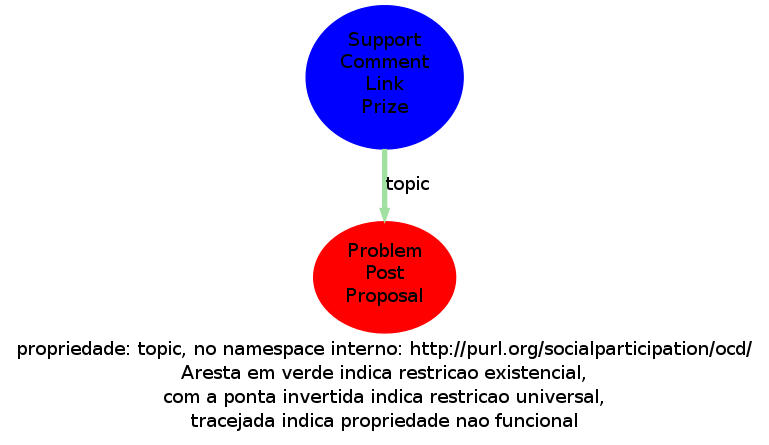
\includegraphics[width=\textwidth]{../figs/topic.png}
  \caption{Figura da propriedade \texttt{ocd:topic}, fruto do método de especificação de ontologias orientado aos dados.}\label{fig:ocdp}
\end{figure}

\begin{figure}[h!]
  \centering
    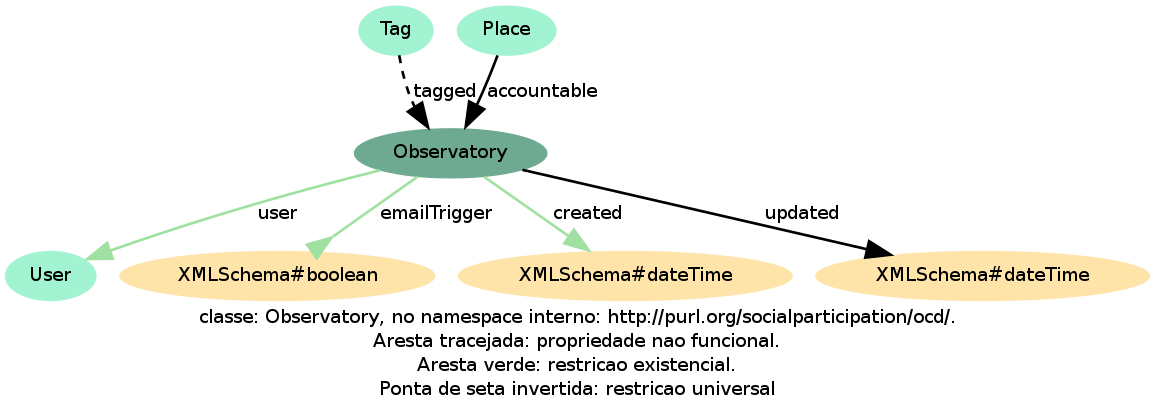
\includegraphics[width=\textwidth]{../figs/Observatory.png}
  \caption{Figura da classe \texttt{ocd:Observatory}, fruto do método de especificação de ontologias orientado aos dados.}\label{fig:ocdc}
\end{figure}

\begin{figure}[h!]
  \centering
    \includegraphics[width=\textwidth]{../figs/OCD_2.png}
  \caption{Figura geral da ontologia \texttt{ocd}, fruto do método de especificação de ontologias orientado aos dados. Para facilitar visualização, visite as imagens diretamente em~\url{https://raw.githubusercontent.com/ttm/ocd/master/imgs/OCD_.png} e~\url{https://raw.githubusercontent.com/ttm/ocd/master/imgs/OCD_2.png}.}\label{fig:ocdg}
\end{figure}


\section{Revisão da OPa}\label{ap:opa}
O primeiro produto desta consultoria envolveu o levantamento de uma ontologia para o Participa, batizada de OPa. Isso ocorreu antes de serem triplificados os dados do Participa.br e antes até mesmo do consultor ter acesso a estes dados. Isso foi bastante proveitoso, pois obrigou a equipe do participa a conceber uma ontologia genérica para portais participativos, centrada nos conceitos de participante, portal participativo e mecanismo participativo. Estes módulos estarão preservados e constam como legado intelectual, uma contribuição da equipe do Participa.br na conceituação da participação social online.

Já depois de feitas estas ontologias do AA e do Cidade Democrática, e depois de ter feito toda a OBS e VBS, atingimos um paradigma apropriado para triplificação dos dados e organização conceitual. Em resumo:
\begin{itemize}
    \item uso de um namespace interno, como \texttt{http://purl.org/socialparticipation/opa}, para a triplificação dos dados, em todas as classes e propriedades. Isso facilita a navegacao e deixa os dados mais organizados, pois no caso extremo de compatibilidade com alguma classe externa, a classe interna assinala a fonte da instância. Um caso extremo desta pertinência é com o derreferenciamento, em que a url \url{http://purl.org/socialparticipation/opa/Participant} lista todos os participantes da OPA, e sua superclasse, \url{http://purl.org/socialparticipation/ops/Participant} apresenta todos os participantes, sejam da OPA, do AA ou do Cidade Democrática.
    \item Relacionamento das triplas com namespaces externos através da ontologia, com as propriedades \texttt{rdfs:subClassOf} e~\texttt{rdfs:subPropertyOf}. Esta implementação pode vir na medida em que a comunidade se apropriar do andamento, pois estas inferências tornam as consultas lentas pela utilização da máquina de inferência em tempo real ou aumentam a quantidade de triplas no caso das inferências offline. Ou seja, nos estágios iniciais, é mais leve e simples não utilizar namespaces externos.
    \item Liberação da ontologia com \emph{blueprints} em imagens. Acréscimo das restrições de classe, e axiomas de pripriedade na medida em que houver utilidade para não enrijecer a estrutura.
\end{itemize}

Neste contexto, além da ontologia disponível no primeiro produto desta consultoria, a OPa conta com as estruturas orientadas aos dados do portal. Este novo módulo está em implementação no momento de entrega deste produto, e poderá ser observado na URL \url{https://github.com/ttm/pnud5/tree/master/opa}.

\section{Revisão da Triplificação do Participa.br}
O script de triplificação disponibilizado no produto 2 foi adaptado para o paradigma explicitado no Apêndice~\ref{ap:opa}. Além disso,
foram acrescentadas à triplificação algumas informações adicionais de usuários e das postagens em si. O script de triplificação está sendo revisado e estará em: \url{http://github.com/ttm/pnud5/opa/triplificaParticipaB.py}.
\newpage
\section{Ontologia e Vocabulário da Biblioteca Social (OBS e VBS)}
Por ocasião do levantamento da Biblioteca (digital e semântica de participação) Social, por iniciativa da SNAS/SG-PR, e com esforços de diversos parceiros, o consultor iniciou uma sequência de entrevistas individuais. Um workshop foi feito na SGPR no dia 20/10/2014 para receber contribuições de parceiros diversos. Além das entrevistas individuais e do workshop, foram consideradas documentações de referência produzidas sobre e pelos mecanismos e instancias de participação social. A PNPS foi considerada separadamente, dada a informatividade do decreto. Todo o processo foi permeado de troca de mensagens entre o consultor e equipes do Particpa.br, UnB, IPEA, SNAS e MP.

Este apêndice expõe estas contribuições e as organizações ontológicas e de vocabulários que delas resultaram.

\subsection{Materiais enviados pela equipe para referência}
Foi considerado um material fruto de articulação da SNAS. O material consiste de documentos produzidos ou referentes às instâncias e mecanismos de participação social e um produto da consultora Carmen Romcy. Este material deu origem a um vocabulário SKOS sobre documentos de participação social, complementar aos obtidos nos apêndices seguintes. 
Veja a Tabela~\ref{tab:ovbs} para o script que escreve o vocabulário SKOS, para os arquivos RDF e para as listagens de termos.

O material em si está no link~\url{https://drive.google.com/file/d/0B7GnkNzm0kxvSTZWWDRyTFkzNm8/view?usp=sharing}.
 O decreto 8.243 é considerado no Apêndice~\ref{ap:pnps}.

\subsection{Entrevistas individuais e workshop}
Especialistas foram entrevistados individualmente para especificações ontológicas iniciais de instâncias de participação social e estão citados junto às instâncias sobre as quais ajudaram junto aos especialistas que contribuíram no workshop.

\subsubsection{Contextualização - Pedro Pontual, Carmen Romcy e Fernando Cruz}
As três entrevistas iniciais foram feitas com o diretor do DPS/SNAS Pedro Pontual, com a consultora Carmen Romcy (ambas no dia no dia 02 de outubro) e com o prof. Fernando Cruz (11 de outubro).

Na ocasião, foram feitas perguntas para contextualizar a OBS e VBS. Estas perguntas incluíam os usos que idealizavam os entrevistados para a biblioteca, possibilidades de alimentação, público alvo, informações disponibilizadas, técnicas e tecnologias.

Dada a extensão deste produto, este conteúdo não foi organizado nem revisado, e os entrevistados não foram contatados para a liberação das anotações destas entrevistas. O consultor manterá uma versão online em~\url{https://docs.google.com/document/d/1jJuzoQzgqPn_FUFVbleXeiKsXHD1Bd0D0O68nXXN7K8/edit?usp=sharing} para os fins deste documento e como registro do processo.

\subsubsection{Especificação das Conferências - Clovis Souza (entrevista), Clovis, Pedro, Fabiano (workshop)}
Materiais dos profs. Fernando Cruz e Carmem Romcy permitiram rascunhos iniciais da ontologia de conferências nacionais. Estes rascunhos foram usados como base para a entrevista feita com o Clovis Souza em dois dias: 30 de setembro e 03 de outubro. Foram revisados os rascunhos iniciais e especificadas relações dos documentos. Foram gerados dois conjuntos de conceitos relacionados ontologicamente e com vocabulário.

O primeiro conjunto é centrado na conferência em si, e os conceitos principais envolvidos. O segundo conjunto é centrado nos documentos e nos resultados das conferências. Veja a Tabela~\ref{tab:ovbs} para os scripts que escrevem as triplas RDF, os arquivos com ontologias OWL e vocabulários SKOS, e diagramas e listagens.

\subsubsection{Especificação dos Conselhos - Paula Pompeu (entrevista)}
No dia 16 de outubro, foi feita uma entrevista com Paula Pompeu para revisar os rascunhos sobre os conselhos nacionais.
Veja a Tabela~\ref{tab:ovbs} para os scripts que escrevem as triplas RDF, os arquivos com ontologias OWL e vocabulários SKOS, e diagramas e listagens.

\subsubsection{Especificação das Ouvidorias - Lígia M. A. Pereira (entrevista), Anjuli Osterne e Paulo Guimarães (workshop)}
No dia 21 de outubro de 2014, foi feita uma entrevista com Lígia Pereira para revistar a ontologia de ouvidorias federais.
Veja a Tabela~\ref{tab:ovbs} para os scripts que escrevem as triplas RDF, os arquivos com ontologias OWL e vocabulários SKOS, e diagramas e listagens.

\subsubsection{Especificação das Consultas públicas - Fernanda Lobato, Valéssio e Silvia (workshop)}
As contribuições dadas no workshop sobre as consultas públicas deram origem a uma ontologia e um vocabulário iniciais, conforme a Tabela~\ref{tab:ovbs}.

\subsubsection{Especificação das Mesas de diálogo - Roberto, Márcia (workshop)}
As contribuições dadas no workshop sobre as mesas de diálogo deram origem a uma ontologia e um vocabulário iniciais, conforme a Tabela~\ref{tab:ovbs}.


\subsection{Decreto 8.243 (PNPS)}\label{ap:pnps}
A observação cuidadosa do decreto 8.243 foi posterior à incorporação de todas as entrevistas individuais, contribuições de workshop e documentos enviados pela SNAS/SGPR. Ao contrário das ontologias anteriores, que eram usadas de base para o vocabulário, foi feito primeiro o vocabulário. Na sequência, a ontologia foi feita com uma nova leitura do decreto. Isso ocorreu após um estudo inicial, em que ontologias por demais detalhadas da PNPS não se mostraram apropriadas para os usos participativos a que se destinavam. Os estudos ficaram no papel, mas podem ser retomados, principalmente caso usos despontem para representações com detalhamento ontológico que contemplem o texto de forma mais minuciosa.

O decreto trata de cada mecanismo e instância de participação social, e uma seleção destas descrições está feita para cada instância e mecanismo. Além disso, há a mesa de monitoramento, que não é descrita diretamente como mecanismo ou instância de participação. Outra parte importante trata das relações que o decreto apresenta que não se referem a nenhum mecanismo ou instância em específico. A PNPS inteira e cada uma destas partes podem ser observadas por diagramas, apontado na Tabela~\ref{tab:ovbs}.

\subsection{Incorporação e registro das contribuições do workshop do dia \\20/Out/2014, sobre a biblioteca (semântica de participação) social}
Todas as contribuições entregues no workshop foram contempladas: ou integradas às OBS e VBS ou anotada com motivo para não estar integrada. As contribuições dos participantes foram escritas à caneta por eles sobre impressões em A4 e A3 dos diagramas das ontologias de conselhos e de conferências e sobre impressões em A4 das listagens dos vocabulários de conferências e conselhos. Fotos de cada uma das folhas com anotações dos participantes em caneta azul ou preta, e anotações do consultor em caneta vermelha, estão online em: \url{https://github.com/ttm/vocabulario-participacao/tree/master/figs/fotos}.

\subsection{Scripts adicionais}
Scripts para fins diversos, todos em \url{https://github.com/ttm/vocabulario-participacao/tree/master/scripts/}:
\begin{itemize}
    \item dspaceVocabLista.py - monta lista XML com todos os conceitos SKOS da VBS, no formato aceito pelo DSpace. Talvez seja útil algum detalhamento neste XML, o que precisa ser avaliado com os usuários/gestores.
    \item tematres.py - monta lista de termos da VBS para importação pelo tematres.
    \item tematresAutoridades.py - monta lista de autoridades da VBS para importação pelo tematres.
    \item triplificaConferencias.py - triplifica a tabela .xls com dados sobre conferências nacionais.
    \item triplificaConselhos.py -  triplifica a tabela .xls com dados sobre conselhos.
    \item vocabTexto.py - utiliza RDF da VBS para fazer os vocabulários em listas simples e enriquecidas de informações.
\end{itemize}

\subsection{Sistematização das instâncias e arquivos principais}\label{ap:sist}


\begin{table}[htpq!]
\vspace{-1cm}
\centering
\caption{Tabela de arquivos da OBS e VBS com o script que escreve os arquivos RDF (seja ontologia OWL ou vocabulário SKOS), o arquivo escrito em RDF/XML e em Turtle, diagramas para as ontologias, listagens para vocabulários, e uma instância do Webprotege com o recurso carregado e aberto para comentários e cópias. Veja os Apêndices~\ref{ap:ut} e~\ref{ap:sist} para mais informações.}
\begin{tabular}{| p{5,5cm} | c | c | c | c | c | }\hline
 {\bf descrição} & {\bf script} & {\bf RDF/XML} & {\bf Turtle} & {\bf diagramas ou listagens} & {\bf wp} \\\hline\hline
vocabulário SKOS do material de referência enviado pela SNAS  & \ref{i:1} & \ref{i:2} & \ref{i:3} & \ref{i:4},~\ref{i:4_1},~\ref{i:5} &~\ref{i:5wp} \\\hline\hline
ontologia OWL das conferências &~\ref{i:6}&~\ref{i:7}&~\ref{i:8}&~\ref{i:9},~\ref{i:10},~\ref{i:11},~\ref{i:11_1}&~\ref{i:11wp} \\
vocabulário SKOS das conferências &~\ref{i:12}&~\ref{i:13}&~\ref{i:14}&~\ref{i:16},~\ref{i:17},~\ref{i:18}&~\ref{i:18wp} \\\hline\hline

ontologia OWL  de documentos e resultados das conferências &~\ref{i:6a}&~\ref{i:7a}&~\ref{i:8a}&~\ref{i:9a},~\ref{i:10a},~\ref{i:11a},~\ref{i:11_1a}&~\ref{i:11awp} \\
vocabulário SKOS de documentos e resultados das conferências &~\ref{i:12a}&~\ref{i:13a}&~\ref{i:14a}&~\ref{i:16a},~\ref{i:17a},~\ref{i:18a}&~\ref{i:18awp} \\\hline\hline

ontologia OWL dos conselhos &~\ref{i:19}&~\ref{i:20}&~\ref{i:21}&~\ref{i:22},~\ref{i:23},~\ref{i:24},~\ref{i:24_1}&~\ref{i:24wp} \\
vocabulário SKOS dos conselhos &~\ref{i:25}&~\ref{i:26}&~\ref{i:27}&~\ref{i:28},~\ref{i:29},~\ref{i:30}&~\ref{i:30wp} \\\hline\hline

ontologia   OWL das  ouvidorias &~\ref{i:31}&~\ref{i:32}&~\ref{i:33}&~\ref{i:34},~\ref{i:35},~\ref{i:36},~\ref{i:37}&~\ref{i:37wp} \\
vocabulário SKOS das ouvidorias &~\ref{i:38}&~\ref{i:39}&~\ref{i:40}&~\ref{i:41},~\ref{i:42},~\ref{i:43}&~\ref{i:43wp} \\\hline\hline

ontologia   OWL  das consultas públicas &~\ref{i:44}&~\ref{i:45}&~\ref{i:46}&~\ref{i:47},~\ref{i:48},~\ref{i:49},~\ref{i:50}&~\ref{i:50wp} \\
vocabulário SKOS das consultas públicas &~\ref{i:51}&~\ref{i:52}&~\ref{i:53}&~\ref{i:54},~\ref{i:55},~\ref{i:56}&~\ref{i:56wp} \\\hline\hline

ontologia   OWL  das mesas de diálogo &~\ref{i:57}&~\ref{i:58}&~\ref{i:59}&~\ref{i:60},~\ref{i:61},~\ref{i:62},~\ref{i:63}&~\ref{i:63wp} \\
vocabulário SKOS das mesas de diálogo &~\ref{i:64}&~\ref{i:65}&~\ref{i:66}&~\ref{i:67},~\ref{i:68},~\ref{i:69}&~\ref{i:69wp} \\\hline\hline

ontologia   OWL  do Decreto 8.243 &~\ref{i:70}&~\ref{i:71}&~\ref{i:72}&~\ref{i:73},~\ref{i:75},{\bf ~\ref{i:76} - \ref{i:76ii} }&~\ref{i:76wp} \\
vocabulário SKOS do Decreto 8.243 &~\ref{i:77}&~\ref{i:78}&~\ref{i:79}&~\ref{i:80},~\ref{i:81},~\ref{i:82}&~\ref{i:82wp} \\\hline\hline

SKOS do vocabulário do IPEA de participação social &~\ref{i:83}&~\ref{i:84}&~\ref{i:85}&~\ref{i:86}&~\ref{i:86wp} \\\hline\hline
\end{tabular}\label{tab:ovbs}
\end{table}
\vspace{1cm}
Links da Tabela~\ref{tab:ovbs}:
{\scriptsize
\begin{enumerate}
    \item \url{https://raw.githubusercontent.com/ttm/vocabulario-participacao/master/scripts/vbsDocumentacaoVBS.py}\label{i:1}
    \item \url{https://raw.githubusercontent.com/ttm/vocabulario-participacao/master/rdf/vbsDocumentacaoVBS.rdf}\label{i:2}
    \item \url{https://raw.githubusercontent.com/ttm/vocabulario-participacao/master/rdf/vbsDocumentacaoVBS.ttl}\label{i:3}
    \item \url{https://raw.githubusercontent.com/ttm/vocabulario-participacao/master/txt/vbsDocumentacaoVBS.txt} \label{i:4}
    \item \url{https://raw.githubusercontent.com/ttm/vocabulario-participacao/master/txt/vbsDocumentacaoVBSPodada.txt}\label{i:4_1}
    \item \url{https://raw.githubusercontent.com/ttm/vocabulario-participacao/master/txt/vbsDocumentacaoVBSPalavras.txt}\label{i:5}
    \item \url{http://webprotege.stanford.edu/#Edit:projectId=cfe287a2-71a7-4f45-9387-5a4ff097647b}\label{i:5wp}

    \item \url{https://raw.githubusercontent.com/ttm/vocabulario-participacao/master/scripts/obsConferencias.py}\label{i:6}
    \item \url{https://raw.githubusercontent.com/ttm/vocabulario-participacao/master/rdf/obsConferencia.owl}\label{i:7}
    \item \url{https://raw.githubusercontent.com/ttm/vocabulario-participacao/master/rdf/obsConferencia.ttl}\label{i:8}
    \item \url{https://raw.githubusercontent.com/ttm/vocabulario-participacao/master/figs/obsConferencia.png}\label{i:9}
    \item \url{https://raw.githubusercontent.com/ttm/vocabulario-participacao/master/figs/obsConferencia.png}\label{i:10}
    \item \url{https://raw.githubusercontent.com/ttm/vocabulario-participacao/master/figs/obsConferencia.png}\label{i:11}
    \item \url{https://raw.githubusercontent.com/ttm/vocabulario-participacao/master/dot/obsConferencia.dot}\label{i:11_1}
    \item \url{http://webprotege.stanford.edu/#Edit:projectId=b9c725ac-e673-443f-97ef-dab340e4a94f}\label{i:11wp}

    \item \url{https://raw.githubusercontent.com/ttm/vocabulario-participacao/master/scripts/vbsConferencias.py}\label{i:12}
    \item \url{https://raw.githubusercontent.com/ttm/vocabulario-participacao/master/rdf/vbsConferencia.rdf}\label{i:13}
    \item \url{https://raw.githubusercontent.com/ttm/vocabulario-participacao/master/rdf/vbsConferencia.ttl}\label{i:14}
    \item \url{https://raw.githubusercontent.com/ttm/vocabulario-participacao/master/txt/vbsConferencia.txt}\label{i:16}
    \item \url{https://raw.githubusercontent.com/ttm/vocabulario-participacao/master/txt/vbsConferenciaPalavras.txt}\label{i:17}
    \item \url{https://raw.githubusercontent.com/ttm/vocabulario-participacao/master/txt/vbsConferenciaPodada.txt}\label{i:18}
    \item \url{http://webprotege.stanford.edu/#Edit:projectId=dd679187-69bf-40b9-a811-26644c75caf2}\label{i:18wp}

 \item \url{https://raw.githubusercontent.com/ttm/vocabulario-participacao/master/scripts/obsConferenciasDocsRes.py}    \label{i:6a}
     \item \url{https://raw.githubusercontent.com/ttm/vocabulario-participacao/master/rdf/obsConferenciaDocsRes.owl}    \label{i:7a}
     \item \url{https://raw.githubusercontent.com/ttm/vocabulario-participacao/master/rdf/obsConferenciaDocsRes.ttl}    \label{i:8a}
    \item \url{https://raw.githubusercontent.com/ttm/vocabulario-participacao/master/figs/obsConferenciaDocsRes.png}    \label{i:9a}
    \item \url{https://raw.githubusercontent.com/ttm/vocabulario-participacao/master/figs/obsConferenciaDocsRes.png}   \label{i:10a}
    \item \url{https://raw.githubusercontent.com/ttm/vocabulario-participacao/master/figs/obsConferenciaDocsRes.png}   \label{i:11a}
     \item \url{https://raw.githubusercontent.com/ttm/vocabulario-participacao/master/dot/obsConferenciaDocsRes.dot} \label{i:11_1a}
     \item \url{http://webprotege.stanford.edu/#Edit:projectId=4f78f256-4f43-4318-b3ee-4395e50a38fd} \label{i:11awp}

\item \url{https://raw.githubusercontent.com/ttm/vocabulario-participacao/master/scripts/vbsConferenciasDocsRes.py}         \label{i:12a}
     \item \url{https://raw.githubusercontent.com/ttm/vocabulario-participacao/master/rdf/vbsConferenciaDocsRes.rdf}        \label{i:13a}
     \item \url{https://raw.githubusercontent.com/ttm/vocabulario-participacao/master/rdf/vbsConferenciaDocsRes.ttl}        \label{i:14a}
     \item \url{https://raw.githubusercontent.com/ttm/vocabulario-participacao/master/txt/vbsConferenciaDocsRes.txt}        \label{i:16a}
     \item \url{https://raw.githubusercontent.com/ttm/vocabulario-participacao/master/txt/vbsConferenciaDocsResPalavras.txt}\label{i:17a}
     \item \url{https://raw.githubusercontent.com/ttm/vocabulario-participacao/master/txt/vbsConferenciaDocsResPodada.txt}  \label{i:18a}
     \item \url{http://webprotege.stanford.edu/#Edit:projectId=523e053a-6d9a-4baf-9ac9-b3c7f4b3f5a3}  \label{i:18awp}

    \item \url{https://raw.githubusercontent.com/ttm/vocabulario-participacao/master/scripts/obsConselhos.py}\label{i:19}
    \item  \url{https://raw.githubusercontent.com/ttm/vocabulario-participacao/master/rdf/obsConselho.owl}\label{i:20}
    \item  \url{https://raw.githubusercontent.com/ttm/vocabulario-participacao/master/rdf/obsConselho.ttl}\label{i:21}
    \item \url{https://raw.githubusercontent.com/ttm/vocabulario-participacao/master/figs/obsConselho.png}\label{i:22}
    \item \url{https://raw.githubusercontent.com/ttm/vocabulario-participacao/master/figs/obsConselho.png}\label{i:23}
    \item \url{https://raw.githubusercontent.com/ttm/vocabulario-participacao/master/figs/obsConselho.png}\label{i:24}
    \item \url{https://raw.githubusercontent.com/ttm/vocabulario-participacao/master/dot/obsConselho.dot}\label{i:24_1}
    \item \url{http://webprotege.stanford.edu/#Edit:projectId=b0e87a16-d33f-4ed4-86bd-e7c288f34215}\label{i:24wp}

    \item \url{https://raw.githubusercontent.com/ttm/vocabulario-participacao/master/scripts/vbsConselhos.py}\label{i:25}
    \item \url{https://raw.githubusercontent.com/ttm/vocabulario-participacao/master/rdf/vbsConselho.rdf}\label{i:26}
    \item \url{https://raw.githubusercontent.com/ttm/vocabulario-participacao/master/rdf/vbsConselho.ttl}\label{i:27}
    \item \url{https://raw.githubusercontent.com/ttm/vocabulario-participacao/master/txt/vbsConselho.txt}\label{i:28}
    \item \url{https://raw.githubusercontent.com/ttm/vocabulario-participacao/master/txt/vbsConselhoPalavras.txt}\label{i:29}
    \item \url{https://raw.githubusercontent.com/ttm/vocabulario-participacao/master/txt/vbsConselhoPodada.txt}\label{i:30}
    \item \url{http://webprotege.stanford.edu/#Edit:projectId=f921bc20-3650-4e64-a7ad-a83b1723b5a9}\label{i:30wp}

    \item \url{https://raw.githubusercontent.com/ttm/vocabulario-participacao/master/scripts/obsOuvidorias.py}\label{i:31}
    \item  \url{https://raw.githubusercontent.com/ttm/vocabulario-participacao/master/rdf/obsOuvidoria.owl}\label{i:32}
    \item  \url{https://raw.githubusercontent.com/ttm/vocabulario-participacao/master/rdf/obsOuvidoria.ttl}\label{i:33}
    \item \url{https://raw.githubusercontent.com/ttm/vocabulario-participacao/master/figs/obsOuvidoria.png}\label{i:34}
    \item \url{https://raw.githubusercontent.com/ttm/vocabulario-participacao/master/figs/obsOuvidoria.png}\label{i:35}
    \item \url{https://raw.githubusercontent.com/ttm/vocabulario-participacao/master/figs/obsOuvidoria.png}\label{i:36}
    \item  \url{https://raw.githubusercontent.com/ttm/vocabulario-participacao/master/dot/obsOuvidoria.dot}\label{i:37}
    \item  \url{http://webprotege.stanford.edu/#Edit:projectId=f8968196-5f12-4b52-acae-9bcd89e75449}\label{i:37wp}

    \item \url{https://raw.githubusercontent.com/ttm/vocabulario-participacao/master/scripts/vbsOuvidorias.py}\label{i:38}
    \item \url{https://raw.githubusercontent.com/ttm/vocabulario-participacao/master/rdf/vbsOuvidoria.rdf}\label{i:39}
    \item \url{https://raw.githubusercontent.com/ttm/vocabulario-participacao/master/rdf/vbsOuvidoria.ttl}\label{i:40}
    \item \url{https://raw.githubusercontent.com/ttm/vocabulario-participacao/master/txt/vbsOuvidoria.txt}\label{i:41}
    \item \url{https://raw.githubusercontent.com/ttm/vocabulario-participacao/master/txt/vbsOuvidoriaPalavras.txt}\label{i:42}
    \item \url{https://raw.githubusercontent.com/ttm/vocabulario-participacao/master/txt/vbsOuvidoriaPodada.txt}\label{i:43}
    \item \url{http://webprotege.stanford.edu/#Edit:projectId=673e6bd0-f814-4d9c-abb5-fc61b377e95e}\label{i:43wp}

 \item \url{https://raw.githubusercontent.com/ttm/vocabulario-participacao/master/scripts/obsConsultas.py}\label{i:44}
    \item  \url{https://raw.githubusercontent.com/ttm/vocabulario-participacao/master/rdf/obsConsulta.owl}\label{i:45}
    \item  \url{https://raw.githubusercontent.com/ttm/vocabulario-participacao/master/rdf/obsConsulta.ttl}\label{i:46}
    \item \url{https://raw.githubusercontent.com/ttm/vocabulario-participacao/master/figs/obsConsulta.png}\label{i:47}
    \item \url{https://raw.githubusercontent.com/ttm/vocabulario-participacao/master/figs/obsConsulta.png}\label{i:48}
    \item \url{https://raw.githubusercontent.com/ttm/vocabulario-participacao/master/figs/obsConsulta.png}\label{i:49}
    \item  \url{https://raw.githubusercontent.com/ttm/vocabulario-participacao/master/dot/obsConsulta.dot}\label{i:50}
    \item  \url{http://webprotege.stanford.edu/#Edit:projectId=d1ebd08c-a88e-48f6-a92c-54664573ba87}\label{i:50wp}

\item \url{https://raw.githubusercontent.com/ttm/vocabulario-participacao/master/scripts/vbsConsultas.py}        \label{i:51}
    \item \url{https://raw.githubusercontent.com/ttm/vocabulario-participacao/master/rdf/vbsConsulta.rdf}        \label{i:52}
    \item \url{https://raw.githubusercontent.com/ttm/vocabulario-participacao/master/rdf/vbsConsulta.ttl}        \label{i:53}
    \item \url{https://raw.githubusercontent.com/ttm/vocabulario-participacao/master/txt/vbsConsulta.txt}        \label{i:54}
    \item \url{https://raw.githubusercontent.com/ttm/vocabulario-participacao/master/txt/vbsConsultaPalavras.txt}\label{i:55}
    \item \url{https://raw.githubusercontent.com/ttm/vocabulario-participacao/master/txt/vbsConsultaPodada.txt}  \label{i:56}
    \item \url{http://webprotege.stanford.edu/#Edit:projectId=c03fba0c-75ff-4382-87c2-c86660cd7228}  \label{i:56wp}

 \item \url{https://raw.githubusercontent.com/ttm/vocabulario-participacao/master/scripts/obsMesasDeDialogo.py}\label{i:57}
    \item  \url{https://raw.githubusercontent.com/ttm/vocabulario-participacao/master/rdf/obsMesaDeDialogo.owl}\label{i:58}
    \item  \url{https://raw.githubusercontent.com/ttm/vocabulario-participacao/master/rdf/obsMesaDeDialogo.ttl}\label{i:59}
    \item \url{https://raw.githubusercontent.com/ttm/vocabulario-participacao/master/figs/obsMesaDeDialogo.png}\label{i:60}
    \item \url{https://raw.githubusercontent.com/ttm/vocabulario-participacao/master/figs/obsMesaDeDialogo.png}\label{i:61}
    \item \url{https://raw.githubusercontent.com/ttm/vocabulario-participacao/master/figs/obsMesaDeDialogo.png}\label{i:62}
    \item  \url{https://raw.githubusercontent.com/ttm/vocabulario-participacao/master/dot/obsMesaDeDialogo.dot}\label{i:63}
    \item  \url{ihttp://webprotege.stanford.edu/#Edit:projectId=b76fbe91-6688-4973-92a1-a77bc09df8eb}\label{i:63wp}

\item \url{https://raw.githubusercontent.com/ttm/vocabulario-participacao/master/scripts/vbsMesasDeDialogo.py}        \label{i:64}
    \item \url{https://raw.githubusercontent.com/ttm/vocabulario-participacao/master/rdf/vbsMesaDeDialogo.rdf}        \label{i:65}
    \item \url{https://raw.githubusercontent.com/ttm/vocabulario-participacao/master/rdf/vbsMesaDeDialogo.ttl}        \label{i:66}
    \item \url{https://raw.githubusercontent.com/ttm/vocabulario-participacao/master/txt/vbsMesaDeDialogo.txt}        \label{i:67}
    \item \url{https://raw.githubusercontent.com/ttm/vocabulario-participacao/master/txt/vbsMesaDeDialogoPalavras.txt}\label{i:68}
    \item \url{https://raw.githubusercontent.com/ttm/vocabulario-participacao/master/txt/vbsMesaDeDialogoPodada.txt}  \label{i:69}
    \item \url{http://webprotege.stanford.edu/#Edit:projectId=a0f33da0-3c37-480e-855c-6a9e544535e2}  \label{i:69wp}

 \item \url{https://raw.githubusercontent.com/ttm/vocabulario-participacao/master/scripts/obsPNPS.py} \label{i:70}
    \item  \url{https://raw.githubusercontent.com/ttm/vocabulario-participacao/master/rdf/obsPNPS.owl}\label{i:71}
    \item  \url{https://raw.githubusercontent.com/ttm/vocabulario-participacao/master/rdf/obsPNPS.ttl}\label{i:72}
    \item \url{https://raw.githubusercontent.com/ttm/vocabulario-participacao/master/figs/obsPNPS.png}\label{i:73}
    \item \url{https://raw.githubusercontent.com/ttm/vocabulario-participacao/master/figs/obsPNPS3.png}\label{i:75}

    \item  \url{https://raw.githubusercontent.com/ttm/vocabulario-participacao/master/dot/obsPNPS.dot}\label{i:76}
    \item  \url{https://raw.githubusercontent.com/ttm/vocabulario-participacao/master/dot/obsPNPS_ambientev.png}\label{i:76b}
    \item  \url{https://raw.githubusercontent.com/ttm/vocabulario-participacao/master/dot/obsPNPS_ambientev2.png}\label{i:76c}
    \item  \url{https://raw.githubusercontent.com/ttm/vocabulario-participacao/master/dot/obsPNPS_ambientev3.png}\label{i:76d}
    \item  \url{https://raw.githubusercontent.com/ttm/vocabulario-participacao/master/dot/obsPNPS_audiencia.png}\label{i:76e}
    \item  \url{https://raw.githubusercontent.com/ttm/vocabulario-participacao/master/dot/obsPNPS_audiencia2.png}\label{i:76f}
    \item  \url{https://raw.githubusercontent.com/ttm/vocabulario-participacao/master/dot/obsPNPS_audiencia3.png}\label{i:76g}
    \item  \url{https://raw.githubusercontent.com/ttm/vocabulario-participacao/master/dot/obsPNPS_comissao.png}\label{i:76h}
    \item  \url{https://raw.githubusercontent.com/ttm/vocabulario-participacao/master/dot/obsPNPS_comissao2.png}\label{i:76i}
    \item  \url{https://raw.githubusercontent.com/ttm/vocabulario-participacao/master/dot/obsPNPS_comissao3.png}\label{i:76j}
    \item  \url{https://raw.githubusercontent.com/ttm/vocabulario-participacao/master/dot/obsPNPS_conferencia.png}\label{i:76k}
    \item  \url{https://raw.githubusercontent.com/ttm/vocabulario-participacao/master/dot/obsPNPS_conferencia2.png}\label{i:76l}
    \item  \url{https://raw.githubusercontent.com/ttm/vocabulario-participacao/master/dot/obsPNPS_conferencia3.png}\label{i:76m}
    \item  \url{https://raw.githubusercontent.com/ttm/vocabulario-participacao/master/dot/obsPNPS_conselho.png}\label{i:76n}
    \item  \url{https://raw.githubusercontent.com/ttm/vocabulario-participacao/master/dot/obsPNPS_conselho2.png}\label{i:76o}
    \item  \url{https://raw.githubusercontent.com/ttm/vocabulario-participacao/master/dot/obsPNPS_conselho3.png}\label{i:76p}
    \item  \url{https://raw.githubusercontent.com/ttm/vocabulario-participacao/master/dot/obsPNPS_consulta.png}\label{i:76q}
    \item  \url{https://raw.githubusercontent.com/ttm/vocabulario-participacao/master/dot/obsPNPS_consulta2.png}\label{i:76r}
    \item  \url{https://raw.githubusercontent.com/ttm/vocabulario-participacao/master/dot/obsPNPS_consulta3.png}\label{i:76s}
    \item  \url{https://raw.githubusercontent.com/ttm/vocabulario-participacao/master/dot/obsPNPS_forumInterconselhos.png}\label{i:76t}
    \item  \url{https://raw.githubusercontent.com/ttm/vocabulario-participacao/master/dot/obsPNPS_forumInterconselhos2.png}\label{i:76u}
    \item  \url{https://raw.githubusercontent.com/ttm/vocabulario-participacao/master/dot/obsPNPS_forumInterconselhos3.png}\label{i:76v}
    \item  \url{https://raw.githubusercontent.com/ttm/vocabulario-participacao/master/dot/obsPNPS_mesa.png}\label{i:76x}
    \item  \url{https://raw.githubusercontent.com/ttm/vocabulario-participacao/master/dot/obsPNPS_mesa2.png}\label{i:76w}
    \item  \url{https://raw.githubusercontent.com/ttm/vocabulario-participacao/master/dot/obsPNPS_mesa3.png}\label{i:76z}
    \item  \url{https://raw.githubusercontent.com/ttm/vocabulario-participacao/master/dot/obsPNPS_mesam.png}\label{i:76aa}
    \item  \url{https://raw.githubusercontent.com/ttm/vocabulario-participacao/master/dot/obsPNPS_mesam2.png}\label{i:76bb}
    \item  \url{https://raw.githubusercontent.com/ttm/vocabulario-participacao/master/dot/obsPNPS_mesam3.png}\label{i:76cc}
    \item  \url{https://raw.githubusercontent.com/ttm/vocabulario-participacao/master/dot/obsPNPS_ouvidoria.png}\label{i:76dd}
    \item  \url{https://raw.githubusercontent.com/ttm/vocabulario-participacao/master/dot/obsPNPS_ouvidoria2.png}\label{i:76ee}
    \item  \url{https://raw.githubusercontent.com/ttm/vocabulario-participacao/master/dot/obsPNPS_ouvidoria3.png}\label{i:76ff}
    \item  \url{https://raw.githubusercontent.com/ttm/vocabulario-participacao/master/dot/obsPNPS_preliminar.png}\label{i:76gg}
    \item  \url{https://raw.githubusercontent.com/ttm/vocabulario-participacao/master/dot/obsPNPS_preliminar2.png}\label{i:76hh}
    \item  \url{https://raw.githubusercontent.com/ttm/vocabulario-participacao/master/dot/obsPNPS_preliminar3.png}\label{i:76ii}

    \item  \url{http://webprotege.stanford.edu/#Edit:projectId=1f8948f8-fa58-490e-9e81-79457c79a4a3}\label{i:76wp}

\item \url{https://raw.githubusercontent.com/ttm/vocabulario-participacao/master/scripts/vbsPNPS.py}         \label{i:77}
    \item \url{https://raw.githubusercontent.com/ttm/vocabulario-participacao/master/rdf/vbsPNPS.rdf}        \label{i:78}
    \item \url{https://raw.githubusercontent.com/ttm/vocabulario-participacao/master/rdf/vbsPNPS.ttl}        \label{i:79}
    \item \url{https://raw.githubusercontent.com/ttm/vocabulario-participacao/master/txt/vbsPNPS.txt}        \label{i:80}
    \item \url{https://raw.githubusercontent.com/ttm/vocabulario-participacao/master/txt/vbsPNPSPalavras.txt}\label{i:81}
    \item \url{https://raw.githubusercontent.com/ttm/vocabulario-participacao/master/txt/vbsPNPSPodada.txt}  \label{i:82}
    \item \url{http://webprotege.stanford.edu/#Edit:projectId=e5c6b505-1c78-4cae-8424-8e628d070da6}  \label{i:82wp}

\item \url{https://raw.githubusercontent.com/ttm/vocabulario-participacao/master/scripts/vbsIPEA.py}         \label{i:83}
    \item \url{https://raw.githubusercontent.com/ttm/vocabulario-participacao/master/rdf/vbsIPEA.rdf}        \label{i:84}
    \item \url{https://raw.githubusercontent.com/ttm/vocabulario-participacao/master/rdf/vbsIPEA.ttl}        \label{i:85}
    \item \url{https://raw.githubusercontent.com/ttm/vocabulario-participacao/master/txt/vbsIPEAPalavras.txt}\label{i:86}
    \item \url{http://webprotege.stanford.edu/#Edit:projectId=11cf0d1a-b13e-43bc-b651-9d95471a692a}\label{i:86wp}
\end{enumerate}
}

\section{Utilização dos dados linkados}\label{ap:ut}

As ontologias mais importantes para este trabalho precisam ser observáveis e anotáveis com facilidade por não especialistas.

Uma primeira opção é aproveitar os dados/triplas disponíveis no endpoint sparql já aberto com uma instância Fuseki/Jena. Este endpoint pode ser acessado via linguagens de scripting para prototipação rápida, como JavaScript, Ruby ou Python, fornecendo interfaces gráficas e web para navegação e análise, com acesso pleno aos dados triplificados via buscas semânticas. Estas possibilidades estão desenvolvidas nos produtos 2, 3 e 4 desta mesma consultoria~\cite{repoProd2, repoProd3, repoProd4}. A OBS e VBS estão disponíveis no endpoint \url{http://200.144.255.210:8082/participacao/query}. Dados do AA, e suas relações ontológicas, estão disponíveis em \url{http://200.144.255.210:8082/aa/query}. Dados do Cidade Democrática, e suas relações ontológicas, estão disponíveis em \url{http://200.144.255.210:8082/cidadedemocratica/query}. Dados do Participa.br, e suas relações ontológidas, estão disponíveis em \url{http://200.144.255.210:8082/participabr/query}. Uma interface geral está em \url{http://200.144.255.210:8082/}. No momento, todos os dados e ontologias estão disponiveis em  \url{http://200.144.255.210:8082/participacao/query} junto à OBS e VBS, para facilitar experimentos.

\subsection{Pubby}
Com desenvolvimento recente no github \url{https://github.com/cygri/pubby}, é talvez o navegador de dados mais conhecido. Parece ser projeto do dig (grupo do Berners-Lee no MIT).
Os testes mostraram que as consultas sparql demoravam demais para o montante de dados triplificados, portanto foram importados os rdfs no pubby diretamente. O arquivo de configuração do pubby está em \url{https://github.com/ttm/vocabulario-participacao/blob/master/auxiliar/config.ttl}.

A url permanente \url{http://purl.org/socialparticipation/} é redirecionada para a instância do pubby, em: \url{http://200.144.255.210:8081/tpubby/page/}. Desta forma, \emph{todos} os conceitos da VBS e classes da OBS podem ser derreferenciados, como na Figura~\ref{fig:derre}. Todos os conceitos, classes e instâncias da OPA, OPS e AA estão também derreferenciados, como na Figura~\ref{fig:aashout}, através do redirecionamento do prefixo \url{http://purl.prg/socialparticipation/} para o endereço \url{http://200.144.255.210:8081/tpubby/page/}, onde opera o pubby.

\begin{figure}[h!]
  \centering
    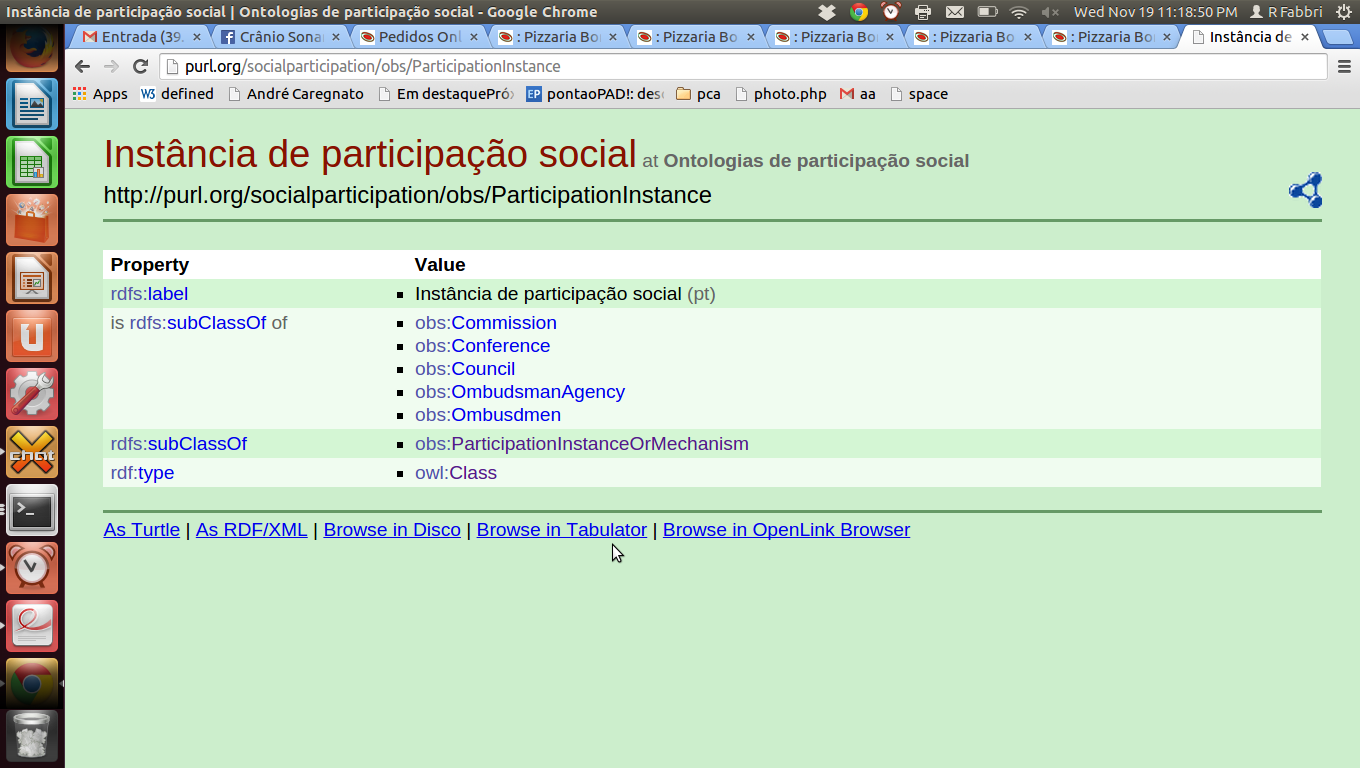
\includegraphics[width=\textwidth]{../figs/derre.png}
  \caption{Derreferenciamento do conceito de Instância de participação através da URI \url{http://purl.org/socialparticipation/obs/ParticipationInstance}.}\label{fig:derre}
\end{figure}

O pubby está operante em uma máquina de pesquisa da nuvem da USP, cuja administração é feita pelo consultor com a permissão de técnicos e docentes do IFSC/USP. Embora útil, a porta não padrão para navegação HTTP impede que a maioria dos gestores públicos federais acessem estes links e derreferenciem as URIs para obter informações sobre o vocábulo, classe ontológica, propriedade que relaciona um objeto a um dado ou outro objeto, instâncias de classes, etc. Colaboradores e funcionários podem estudar e testar o pubby e outras intefaces para dados linkados para que sejam disponibilizados servicos melhores e mais diversificados.

\subsection{Webprotege}

Este software permite que as ontologias e vocabulários estejam online e comentáveis, além da criação e edição de ontologias na própria interface.

Nas tentativas do consultor de levantar uma instância deste software, foram encontrados alguns roteiros incompletos na wiki e conflitos do java. Dados os resultados instáveis e especificidades técnicas, o consultor subiu os arquivos no webprotege instalado e disponibilizado pela equipe da Stanford que desenvolve o webprotege. 
No presente momento, apenas o consultor pode editar, mas todos podem comentar ou fazer cópias dos vocabulários e ontologias. Veja a Tabela~\ref{tab:ovbs} para os links.





%\section{Cartas ao poder público federal}
%\subsection{Religião e cultura livre}
%\subsection{Autoritarismo/preconceito e rede social}
%\subsection{Pesquisa e desenvolvimento para participação}
%\subsection{Subsídios para pulverizar a participação e qualificá-la}

%\section{Técnicas de difusão de informação}
%\subsection{Reprodução do experimento apocalíptico de 2012}




\end{document}
